% -----------------------------------------------
% Template for ISMIR Papers
% 2016 version, based on previous ISMIR templates

% Requirements :
% * 6+1 page length maximum
% * 2MB maximum file size
% * Copyright note must appear in the bottom left corner of first page
% (see conference website for additional details)
% -----------------------------------------------

\documentclass{article}
\usepackage{ismir,amsmath,cite}
\usepackage{graphicx}
\usepackage{color}
\usepackage{booktabs}

% Title.
% ------
\title{Automatic Music Transcription \conferenceyear}

% Note: Please do NOT use \thanks or a \footnote in any of the author markup

% Single address
% To use with only one author or several with the same address
% ---------------
%\oneauthor
% {Names should be omitted for double-blind reviewing}
% {Affiliations should be omitted for double-blind reviewing}

% Two addresses
% --------------
%\twoauthors
%  {First author} {School \\ Department}
%  {Second author} {Company \\ Address}

%% To make customize author list in Creative Common license, uncomment and customize the next line
%  \def\authorname{First Author, Second Author} 


% Three addresses
% --------------
\threeauthors
  {Nora Huang} {Department of Computer Science\\
University of Victoria\\
Victoria, B.C, Canada \\ {\tt norah@uvic.ca}}
  {Aazim Lakhani} {Department of Computer Science\\
University of Victoria\\
Victoria, B.C, Canada \\ {\tt aazimlakhani@uvic.ca}}
  {Parul Smaddar} {Department of Computer Science\\
University of Victoria\\
Victoria, B.C, Canada \\ {\tt parulsmaddar@gmail.com}}

%% To make customize author list in Creative Common license, uncomment and customize the next line
%  \def\authorname{First Author, Second Author, Third Author} 

% Four or more addresses
% OR alternative format for large number of co-authors
% ------------
%\multauthor
%{First author$^1$ \hspace{1cm} Second author$^1$ \hspace{1cm} Third author$^2$} { \bfseries{Fourth author$^3$ \hspace{1cm} Fifth author$^2$ \hspace{1cm} Sixth author$^1$}\\
%  $^1$ Department of Computer Science, University , Country\\
%$^2$ International Laboratories, City, Country\\
%$^3$  Company, Address\\
%{\tt\small CorrespondenceAuthor@ismir.edu, PossibleOtherAuthor@ismir.edu}
%}
%\def\authorname{First author, Second author, Third author, Fourth author, Fifth author, Sixth author}


\sloppy % please retain sloppy command for improved formatting

\begin{document}

%
\maketitle
%
\begin{abstract}
The objective of this project is to evaluate the accuracy of various models to perform automatic music transcription by extracting features from the audio music and applying different classifiers to get the note. Through this initiative we plan to focus at transcription on certain music instruments. Furthermore, only the main instrument of the polyphonic music will be transcribed.
\end{abstract}
%
\section{Introduction}\label{sec:introduction}
The dataset for this project will collected through MIDI Aligned Piano Sounds (MAPS) , Isophonics Annotations , KSN Database to name a few. The sources claim the data is used for transcriptions of both monophonic \& polyphonic instruments. The datasets are annotated \& we would evaluate the data to use music relevant for this project.  \\\\
Then acoustics features such as Zero Crossing Rate, Autocorrelation, YIN metrics for time domain \& FFT , STFT , Spectrogram , cestrum metrics, spectral flux for the frequency domain would be used to extract notes from audio music. \\\\
The extracted features will be used as input to the classifiers for note transcription. Different classifiers, such as K-NN, Logistic Regression, Stochastic Gradient Descent, Support Vector Machines (SVM) would be evaluated for accuracy. Features would be combined together to give better accuracy on real world data.\\
\\
Marsyas would be used as the framework for acoustic features extraction. Python \& Scikit-learn would be used to prepare the learning model, which would eventually, transcribe.  

\begin{figure}
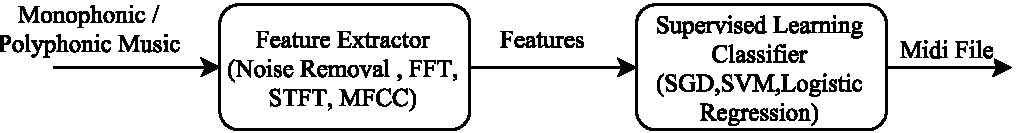
\includegraphics[scale=.55]{System_Flow_Diagram}
\\System Flow Diagram
\end{figure}

\subsection{Timeline}\label{subsec:Timeline}
We make 4 milestone for the whole project, for each task there will be two responsible team member for it, one as primary while the other as secondary. Please find the detail of the milestone in Table \ref{table1}
\begin{table}[h]
 \begin{center}
\begin{tabular}{c|c|c|c|c}
        \toprule
         MileStones & Deadline & Tasks & Primary & Secondary  \\
       \midrule
        %\midline
        MileStone1 & March 6 & Dataset & Aazim & Nora \\
         &  & Features   & Parul & Nora \\
         &  & Classifier  & Nora & Aazim \\
        \midrule
        MileStone2 & March 13 & Train & TBD  &  TBD    \\
        \midrule
        MileStone3 & March27 & Testing & TBD &  TBD   \\
                \midrule
        MileStone4 & March30 & Report &TBD  & TBD    \\
        \bottomrule
        %Note. Values are given as mean $\pm$ SD.   &                      &                     \\
\end{tabular}
\end{center}
 \caption{Milestones}
 \label{table1}
\end{table}


\subsection{Role of team member}\label{subsec:Role of team member}
Nora: Architecture design, team management, coding\\
Aazim: Training \& testing with different combinations of classifiers \& features\\
Parul: Work on audio processing \& feature extraction. 
 
%
\section{Dataset}\label{sec:Dataset}
We obtained data for both monophonic and polyphonic sounds through MAPS. We're also in the process of having data from Isophonics Annotations \& KSN Database. 

\section{Acoustic features for training}\label{sec:features}
Time Domain : Zero Crossing Rate, Autocorrelation, YIN metrics Frequency Domain : FFT , STFT , Spectrogram , cestrum metrics, spectral flux.

\section{Classifiers}\label{sec:Classifiers}
Stochastic Gradient Descent, Logistic Regression, Support Vector Machines


\section{Result}\label{sec:Result}
This would comprise of the collection of features, classifiers used to give the highest level accuracy. Various combinations would be tried, but only the one's that generalize well, would be mentioned in the result. 

\section{Conclusion}\label{sec:Conclusion}
Basic on the result we should be able to figure out which combination is best for automatic music transcription.



\section{References}


% For bibtex users:
\bibliography{ISMIRtemplate}

% For non bibtex users:
%\begin{thebibliography}{citations}
%
%\bibitem {Author:00}
%E. Author.
%``The Title of the Conference Paper,''
%{\it Proceedings of the International Symposium
%on Music Information Retrieval}, pp.~000--111, 2000.
%
%\bibitem{Someone:10}
%A. Someone, B. Someone, and C. Someone.
%``The Title of the Journal Paper,''
%{\it Journal of New Music Research},
%Vol.~A, No.~B, pp.~111--222, 2010.
%
%\bibitem{Someone:04} X. Someone and Y. Someone. {\it Title of the Book},
%    Editorial Acme, Porto, 2012.
%
%\end{thebibliography}

\end{document}
